\documentclass[conference]{IEEEtran}

% ── Packages ──────────────────────────────────────────────────────────────
\usepackage{amsmath,amssymb}
\usepackage{graphicx}
\usepackage{booktabs}
\usepackage{algorithm}
\usepackage{algorithmic}
\usepackage{cite}
\usepackage{xcolor}
\usepackage[caption=false,font=footnotesize]{subfig}
\usepackage{placeins}
\usepackage{url}
\usepackage[hidelinks]{hyperref}


% ── Macros ────────────────────────────────────────────────────────────────
\newcommand{\todo}[1]{\textcolor{red}{\textbf{[TODO: #1]}}}
\newcommand{\nqubits}{n}
\newcommand{\shots}{s}

% ── Title Block ───────────────────────────────────────────────────────────
\title{Polynomial-Resource Classification of Quantum Circuit Families via Classical Shadows}

\author{
\IEEEauthorblockN{Andrew Maciejunes}
\IEEEauthorblockA{
Virginia Modeling, Analysis and Simulation Center\\
Old Dominion University\\
Norfolk, VA, USA\\
amacieju@odu.edu
}
\and
\IEEEauthorblockN{Ross Gore}
\IEEEauthorblockA{
Center for Secure and Intelligent Critical Systems\\
Old Dominion University\\
Norfolk, VA, USA\\
rgore@odu.edu
}
}

\begin{document}

\maketitle

\begin{abstract}
We compare three polynomial-resource measurement strategies---$Z$-basis-only, multi-basis ($Z$/$X$/$Y$), and classical shadows---for classifying three quantum circuit families: IQP, Clifford, and Clifford$+T$.
Contrary to the initial hypothesis, $Z$-only measurements outperform both multi-basis and classical shadows across all qubit counts and all four classifiers evaluated.
The best result is a Random Forest accuracy of $0.92$ at 4--5 qubits under $Z$-only, against $0.87$ for multi-basis and $0.65$ for shadows.
All three strategies collapse to near-chance accuracy ($\approx 0.33$) above approximately 12 qubits under the quadratic shot budget $\shots = 16\nqubits^2$.
These findings indicate that the discriminative signal between IQP, Clifford, and Clifford$+T$ families is concentrated in $Z$-basis correlations, consistent with the diagonal gate structure of IQP circuits, and that the additional Pauli correlator types accessed by multi-basis measurements and classical shadows carry no compensating discriminative power for this task.
\end{abstract}

\begin{IEEEkeywords}
classical shadows, quantum circuit families, IQP circuits, Clifford circuits, polynomial resources, distribution classification, Pauli correlators, quantum machine learning
\end{IEEEkeywords}

\section{Introduction}
\label{sec:intro}


A fundamental question in quantum information is whether the output distributions of quantum circuits, distributions that cannot be efficiently represented classically, can be meaningfully characterized using only polynomially many measurements. 
Quantum state tomography, originally proposed by Vogel and Risken (1989) \cite{vogel1989determination} and first demonstrated experimentally by Smithey et al. (1993) \cite{smithey1993measurement}, provides a complete reconstruction of the quantum state but at prohibitive cost. 
Haah et al. (2016) \cite{haah2016sample} rigorously established this cost with a lower bound of $\Omega(d^2/\delta)$ copies, where d is the Hilbert space dimension and $\delta$ is the desired precision. 
Since $d = 2^n$ for an n-qubit system, full tomography requires exponentially many measurements in the number of qubits, rendering it infeasible for systems of practical interest. 
This exponential barrier motivates the search for protocols that extract meaningful information about quantum states without full reconstruction.

Quantum circuit families provide a principled testbed for this question.
IQP, Clifford, and Clifford$+T$ circuits produce distributions with qualitatively different statistical signatures, rooted in their distinct computational complexity properties.
Clifford circuits are classically simulable; IQP sampling is believed to be classically hard under plausible complexity-theoretic conjectures%~\cite{Bremner2016}
; Clifford$+T$ circuits interpolate between the two.
If these families can be distinguished with polynomially many measurements, it suggests that their distributional signatures are encoded in low-order statistics that a polynomial measurement protocol can access.

The key methodological challenge is choosing the right measurement protocol.
Measuring in a single basis ($Z$-only) gives access to $ZZ$ correlators but misses the $X$ and $Y$ components of the Pauli correlation structure.
Measuring in three global bases ($Z$, $X$, $Y$) recovers $ZZ$, $XX$, and $YY$ correlators but requires $3\times$ the shot budget and still misses mixed-basis correlators ($XY$, $XZ$, $YZ$).
Classical shadows%~\cite{Huang2020}
resolve this: by applying a random single-qubit Clifford rotation to each qubit before measurement, all six two-qubit Pauli correlators can be estimated from a single unified measurement protocol, with sample complexity $O(\nqubits^2)$---matching the shot budget required for any individual correlator type.

\paragraph*{Contributions}
\begin{itemize}
    \item An empirical demonstration that $Z$-only measurement outperforms multi-basis and classical shadows for classifying IQP, Clifford, and Clifford$+T$ circuit families, inverting the original hypothesis that richer Pauli correlation structure would benefit classification.
    \item Evidence that the discriminative signal between these three circuit families is concentrated in $Z$-basis correlations rather than in the mixed-basis Pauli correlators accessed by shadows, consistent with the diagonal computational-basis structure of IQP circuits.
    \item Characterization of a scaling collapse near 12 qubits at which all polynomial strategies degrade to near-chance performance under the quadratic shot budget $\shots = 16\nqubits^2$, establishing a practical limit for this feature set and shot scaling law.
\end{itemize}

\section{Background}
\label{sec:background}

\subsection{Circuit Families as Distribution Classes}

We consider three quantum circuit families that span a range of computational complexity.

\paragraph{Clifford circuits}
Generated by $\{H, S, \mathrm{CNOT}\}$, Clifford circuits are efficiently simulable classically via the stabilizer formalism.%~\cite{Gottesman1998}
Their output distributions possess structured pairwise correlations reflecting the underlying stabilizer group geometry.

\paragraph{Clifford$+T$ circuits}
Adding $T = \mathrm{diag}(1, e^{i\pi/4})$ yields a universal gate set.%~\cite{Boykin2000}
Sufficient $T$-gate density breaks the stabilizer structure and moves the circuit outside the efficiently simulable regime, producing a distributional signature intermediate between Clifford and IQP.

\paragraph{IQP circuits}
Instantaneous Quantum Polynomial circuits apply diagonal gates in the computational basis, sandwiched by Hadamard layers.%~\cite{Shepherd2009}
Classical hardness of IQP sampling is supported by complexity-theoretic arguments%~\cite{Bremner2016}
, and their parity structure produces a distributional fingerprint qualitatively distinct from the Clifford family.

\subsection{Classical Shadows}

Classical shadows%~\cite{Huang2020}
provide an efficient protocol for estimating many properties of a quantum state from a single randomized measurement dataset.
For each measurement shot, a random single-qubit unitary $U_i$ is applied to each qubit $i$ before measurement in the computational basis, and the rotation choice is recorded alongside the outcome.
The measurement channel can then be inverted classically to produce unbiased estimators for arbitrary observables.

For a single-qubit Pauli $P_i \in \{X, Y, Z\}$, the shadow estimator is:
\begin{equation}
\hat{P}_i = 3 \cdot (-1)^{b_i} \cdot \mathbf{1}[U_i \text{ matches } P_i\text{'s basis}],
\end{equation}
where the factor of 3 corrects for the $1/3$ probability of any given basis being selected.
For a two-qubit correlator $P_i P_j$, the estimator is the product of single-qubit estimators, yielding a factor of $9$ and requiring both $U_i$ and $U_j$ to match their respective Pauli bases.

The connected correlator $\langle P_i P_j \rangle_c = \langle P_i P_j \rangle - \langle P_i \rangle \langle P_j \rangle$ can be estimated by combining single- and two-qubit shadow estimators.
For $K$ Pauli operators, the required number of shadows scales as $O(K / \varepsilon^2)$ for bounded observables, independent of system size.%~\cite{Huang2020}
For all $6 \cdot \binom{\nqubits}{2}$ two-qubit Pauli correlators, this yields a total shot cost of $O(\nqubits^2 / \varepsilon^2)$---polynomial in $\nqubits$.

\FloatBarrier
\begin{figure*}[!ht]
\centering
\subfloat[Clifford]{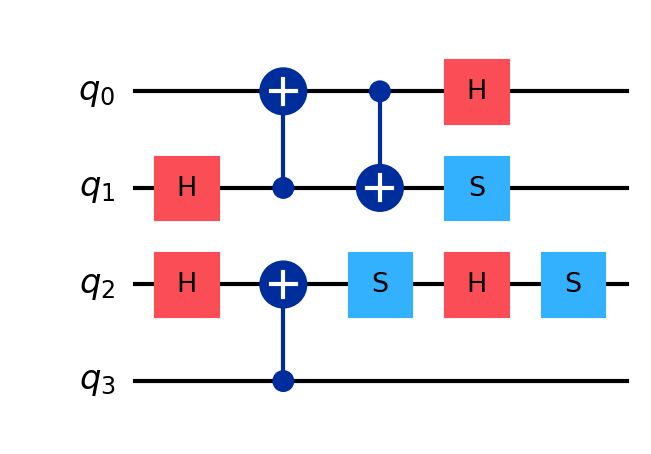
\includegraphics[width=0.25\textwidth,height=4cm,keepaspectratio]{images/clifford.png}%
\label{fig:clifford}}
\hfil
\subfloat[Clifford$+T$]{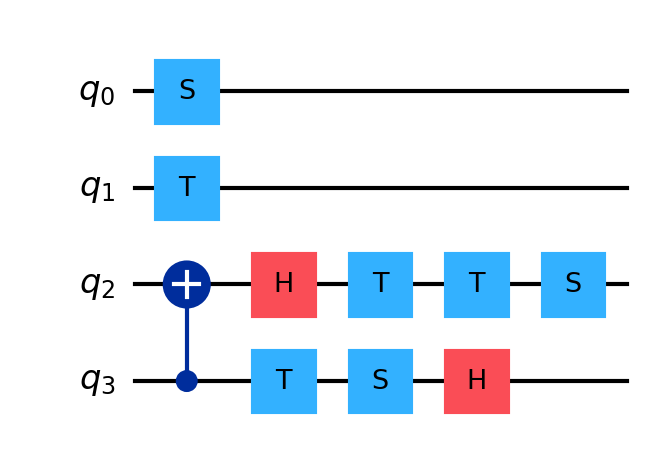
\includegraphics[width=0.25\textwidth,height=4cm,keepaspectratio]{images/cliffordT.png}%
\label{fig:cliffordT}}
\hfil
\subfloat[IQP]{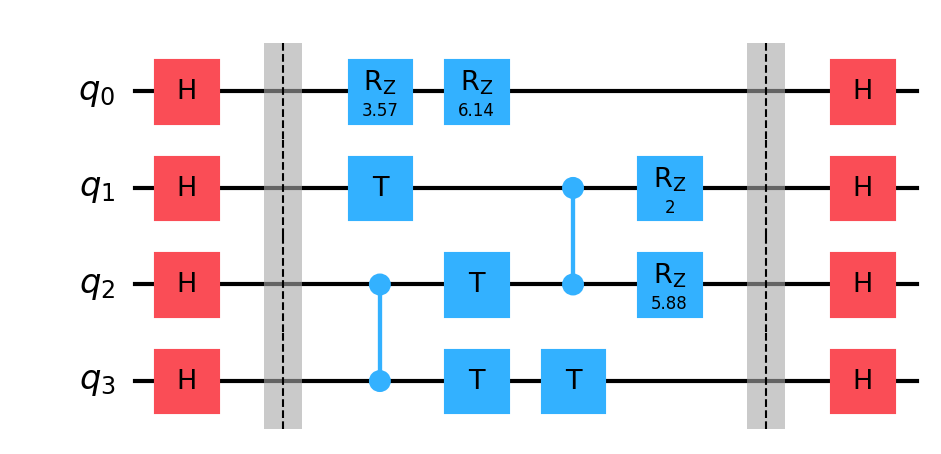
\includegraphics[width=0.35\textwidth,height=4cm,keepaspectratio]{images/IQP.png}%
\label{fig:iqp}}
\caption{We illustrate an example Clifford, Clifford$+T$, and IQP circuit for the reader with four
qubits and $N_c$ = 10. (a) The Clifford circuit is comprised of gates from the clifford gate 
as defined above. (b) We observe a disproportionate amount of T gates for the Clifford+T example. This is done to 
ensure distinctness from the Clifford circuit family. (c) We show an example IQP circuit. It is 
clear that $N_c$ for IQP circuits refers to the number of operations between the Hadamard gates.}
\label{fig:circuit_families}
\end{figure*}
\FloatBarrier

\subsection{Distribution Classification}

Distribution testing and quantum state discrimination provide the theoretical foundations for circuit family classification.
Classical distribution testing asks whether two sample sequences were drawn from the same distribution, with sample complexity that depends on the alphabet size and closeness notion~\cite{Canonne2020}.
In the quantum setting, quantum state discrimination minimizes the probability of misidentifying one of several candidate states given a fixed number of copies~\cite{Barnett2009}, while quantum hypothesis testing establishes error exponents for distinguishing between two states in the asymptotic copy limit~\cite{Audenaert2007}.
These frameworks are information-theoretically tight but assume access to the full quantum state; when only classical measurement outcomes are available the problem reduces to distinguishing between high-dimensional probability distributions from samples.

More directly related is the body of work on circuit fingerprinting and spoofing detection.
Aaronson and Chen~\cite{AaronsonChen2017} propose linear cross-entropy benchmarking as a statistical test for quantum supremacy claims, exploiting the anticorrelation between a classical simulator's probability assignments and typical bitstring frequencies.
Barak et al.~\cite{BarakEtAl2021} show that low-degree polynomial estimators cannot efficiently distinguish random quantum circuit outputs from uniform noise at large system size, establishing hardness results for feature-based discrimination.
Hangleiter et al.~\cite{HangleiterEtAl2019} study anticoncentration and show that IQP and random circuit families exhibit qualitatively different concentration behavior, a property reflected in Hamming-weight statistics.
The present work complements these results by providing a systematic empirical comparison of $Z$-only, multi-basis, and classical shadows measurement strategies for circuit family classification, and is, to our knowledge, the first study to directly benchmark all three strategies against each other on the IQP, Clifford, and Clifford$+T$ families across a range of qubit counts.

\section{Methods}
\label{sec:methods}

\subsection{Circuit Generation}

We use the Qiskit SDK \cite{qiskit2024} for all of our research. Using Qiskit, we craft random circuits 
for each of the three previously mentioned circuit families, Clifford, Clifford$+T$, and IQP circuits.
For the first two groups, we define a value $N_c$, which is the number of gates in a given circuit. We
then apply $N_c$ randomly selected gates from the appropriate circuit family to act on randomly selected 
qubits. For the Clifford family of circuits, each gate has an equal chance of being selected. For the 
Clifford$+T$ family, the gates have chances of being selected as outlined in Table\ref{tab:cliffordT_gate_distros}.
The qubit(s) each gate acts on is selected randomly with no preference to any particular qubit, except 
in the case of two qubit gates, where the control and target must be different.

\begin{table}[htbp]
\centering
\label{tab:cliffordT_gate_distros}
\caption{Clifford$+T$ gate selection probabilities. All other families used equal probabilities.}
\begin{tabular}{|c|c|}\hline
\textbf{Gate} & \textbf{Probability} \\ \hline
 S & 0.2 \\ \hline
 CNOT & 0.2 \\ \hline
 H & 0.2 \\ \hline
 T & 0.4 \\ \hline

\end{tabular}

\end{table}

Instantaneous Quantum Polynomial (IQP) circuits are created simiiarly. The only difference, beside the 
gate set used, is that the operator $H^{\bigotimes n}$ is applied at the beginning and end of the circuit, as 
shown in Figure~\ref{fig:circuit_families}, where n is the number of qubits. We scale the number of qubits from 4 up to 20 qubits. At each qubit count, we generate 1000 circuits of each 
type.

\begin{table}[htbp]
\centering
\caption{Experimental parameter sweep.}
\label{tab:sweep}
\begin{tabular}{ll}
\toprule
\textbf{Parameter} & \textbf{Values} \\
\midrule
Circuit families & IQP, Clifford, Clifford$+T$ \\
Qubit counts & 4--20 \\
Shot budget & $16\nqubits^2$ (quadratic) \\
Circuits per family per qubit count & 1000 \\
Operations per circuit & 1000 \\
Simulator & Qiskit Aer (statevector, GPU) \\
Measurement strategies & $Z$-only, multi-basis, shadows \\
\bottomrule
\end{tabular}
\end{table}

\subsection{Shot Budget Design}
\label{sec:shots}

The estimation cost of a statistical feature determines the minimum shot budget needed to estimate it reliably.

\paragraph{Polynomial-cost features}
The Hamming-weight histogram bins all $2^\nqubits$ outcomes into $\nqubits + 1$ weight classes, requiring $O(\nqubits / \varepsilon^2)$ shots.
Single-qubit marginals $P(x_i = 1)$ and parity bias require $O(\nqubits / \varepsilon^2)$ and $O(1/\varepsilon^2)$ shots respectively.
Connected two-qubit Pauli correlations across all $\binom{\nqubits}{2}$ pairs require $O(\nqubits^2 / \varepsilon^2)$ shots in total for any single correlator type (e.g., $ZZ$, $XX$, $YY$).
By the classical shadows result%~\cite{Huang2020}
, \emph{all} $6\binom{\nqubits}{2}$ two-qubit Pauli correlators ($ZZ$, $XX$, $YY$, $XY$, $XZ$, $YZ$) can be estimated simultaneously at the same $O(\nqubits^2 / \varepsilon^2)$ cost using the shadow protocol.

\paragraph{Excluded exponential-cost features}
The purpose of this work is to classify quantum circuit families using only polynomial measurement resources.
If exponential resources were available, full quantum state tomography could exactly reconstruct the output distribution, rendering classification trivial.
In that vein, several prominent statistical measures are excluded from our feature set due to their exponential shot requirements:
Shannon entropy $H = -\sum_x \hat{p}(x)\log_2 \hat{p}(x)$, which requires $O(2^\nqubits / \nqubits)$ shots because the empirical frequency estimator is biased whenever bitstrings go unobserved;
collision probability $\mathcal{C} = \sum_x p(x)^2$, which requires $O(2^{\nqubits/2})$ shots via the birthday problem threshold;
R\'{e}nyi entropies of order $\alpha \neq 1$, which share the same exponential sampling barrier;
and total variation distance to uniformity, which requires observing a representative fraction of the $2^\nqubits$ outcomes.
All such features are incompatible with the polynomial-resource constraint central to this work and are therefore disregarded.

\paragraph{Quadratic shot scaling}
The most expensive retained features are the two-qubit Pauli correlators, requiring $O(\nqubits^2)$ shots.
We adopt a quadratic shot scaling law $\shots = \lambda \nqubits^2$, where $\shots$ is the total shot budget, $\nqubits$ is the number of qubits, and $\lambda$ is a constant prefactor controlling the statistical quality of the estimators.
We arbitrarily set $\lambda = 16$, giving 256 shots at $\nqubits = 4$ and 6400 shots at $\nqubits = 20$.
For the multi-basis strategy, each of the three basis runs receives $\shots / 3$ shots; the total shot budget remains $\shots = \lambda\nqubits^2$.

\subsection{Measurement Strategies}
\label{sec:strategies}

We compare three measurement protocols, each operating within the same $\shots = 16\nqubits^2$ total shot budget.

\paragraph{$Z$-only baseline}
All shots are taken in the computational basis.
Features extracted: Hamming-weight histogram, $Z$-basis single-qubit marginals, parity bias, and all-pairs connected $ZZ$ correlations.
This is the minimal polynomial-resource strategy and serves as the baseline.

\paragraph{Multi-basis}
Shots are divided equally among three global basis rotations: identity ($Z$ basis), Hadamard on all qubits ($X$ basis), and $S^\dagger H$ on all qubits ($Y$ basis), with $\shots/3$ shots per basis.
Features extracted: Hamming-weight histogram, $Z$/$X$/$Y$ single-qubit marginals, parity bias, and all-pairs connected $ZZ$, $XX$, and $YY$ correlations.
This gives three of the six Pauli pair correlator types at the same total shot cost, at the expense of $3\times$ fewer shots per basis run.
Mixed-basis correlators ($XY$, $XZ$, $YZ$) are not accessible with global rotations.

\paragraph{Classical shadows}
For each of the $\shots$ measurement shots, a random basis ($Z$, $X$, or $Y$) is independently selected for each qubit, and the circuit is measured after applying the corresponding single-qubit rotation.
All six two-qubit Pauli correlator types ($ZZ$, $XX$, $YY$, $XY$, $XZ$, $YZ$) are estimated from the resulting shadow dataset using the unbiased shadow estimators described in Section~\ref{sec:background}.
This achieves the full Pauli correlation structure at the same total shot budget as the $Z$-only baseline.

\subsection{Feature Extraction}
\label{sec:features}

\paragraph{$Z$-only features}
The feature vector concatenates: Hamming-weight histogram ($\nqubits+1$ values), $Z$-marginals ($\nqubits$ values), parity bias (1 value), and all-pairs $ZZ$ connected correlations ($\binom{\nqubits}{2}$ values):
\begin{equation}
d_{\text{Z}} = (\nqubits+1) + \nqubits + 1 + \tfrac{\nqubits(\nqubits-1)}{2} = \tfrac{\nqubits^2 + 3\nqubits + 4}{2}.
\end{equation}
This grows as $O(\nqubits^2)$, dominated by the all-pairs $ZZ$ term.

\paragraph{Multi-basis features}
The feature vector extends the $Z$-only set by appending $X$-marginals and all-pairs $XX$ correlations, then $Y$-marginals and all-pairs $YY$ correlations:
\begin{equation}
d_{\text{MB}} = d_{\text{Z}} + 2\nqubits + \nqubits(\nqubits-1) = O(\nqubits^2).
\end{equation}

\paragraph{Shadow features}
The feature vector concatenates $Z$/$X$/$Y$ single-qubit expectations ($3\nqubits$ values) and all six Pauli pair connected correlations across all $\binom{\nqubits}{2}$ pairs ($6 \cdot \binom{\nqubits}{2}$ values):
\begin{equation}
d_{\text{S}} = 3\nqubits + 6 \cdot \tfrac{\nqubits(\nqubits-1)}{2} = 3\nqubits^2.
\end{equation}
All three feature vectors scale as $O(\nqubits^2)$, consistent with the polynomial-resource design goal.

\subsection{Classification Pipeline}

We evaluate four classifiers from scikit-learn%~\cite{scikit-learn}
: Logistic Regression (L-BFGS, \texttt{max\_iter}=1000), Decision Tree (unlimited depth), Random Forest (100 estimators), and Support Vector Machine (RBF kernel).
Data are split 80/20 train/test.
Accuracy is reported as the fraction of correctly classified test samples.
Each classifier is independently trained and evaluated for each measurement strategy and qubit count.

\paragraph{Logistic Regression}
Logistic Regression models the log-odds of class membership as a linear function of the input features.
Given feature vector $\mathbf{x}$, the probability assigned to class $k$ is
$P(y=k \mid \mathbf{x}) = \mathrm{softmax}(\mathbf{W}\mathbf{x} + \mathbf{b})_k$,
and parameters $\mathbf{W}, \mathbf{b}$ are fit by minimizing cross-entropy via L-BFGS.
The decision boundary is a hyperplane in feature space, making the model fast to train and easy to interpret, but limited to linearly separable classes.

\paragraph{Decision Tree}
A Decision Tree recursively partitions the feature space by selecting, at each node, the feature threshold that maximises the reduction in Gini impurity among the training samples reaching that node.
Predictions for a new sample are made by routing it through the learned splits to a leaf, where the majority class label is returned.
With unlimited depth, the tree can perfectly partition any finite training set, capturing highly non-linear boundaries at the cost of a tendency to overfit.
Unlike Logistic Regression, the decision boundary is piecewise axis-aligned rather than a single hyperplane.

\paragraph{Random Forest}
A Random Forest is an ensemble of decision trees, each trained on an independently drawn bootstrap sample of the training data.
At every split, each tree considers only a random subset of features, decorrelating the trees and reducing variance relative to a single deep tree.
The final prediction is the majority vote across all 100 trees.
Random Forest therefore inherits the non-linear expressivity of individual trees while substantially improving generalisation, at the cost of reduced interpretability compared to a single tree.

\paragraph{Support Vector Machine}
A Support Vector Machine (SVM) finds the maximum-margin separating hyperplane in a (possibly kernel-lifted) feature space.
We use the Radial Basis Function (RBF) kernel $K(\mathbf{x}, \mathbf{x}') = \exp(-\gamma\|\mathbf{x}-\mathbf{x}'\|^2)$, which implicitly maps inputs into an infinite-dimensional space, allowing highly non-linear decision boundaries.
Only the support vectors --- the training samples closest to the margin --- determine the boundary, making SVMs effective in high-dimensional settings where the number of features is large relative to the number of samples.

\paragraph{Key differences}
The four classifiers span two primary axes of variation.
First, \emph{linearity}: Logistic Regression assumes a linear boundary, while the other three can represent non-linear separations.
Second, \emph{variance--bias trade-off}: a single Decision Tree has low bias but high variance; Random Forest reduces variance through ensemble averaging; SVMs control both through the margin objective and the choice of kernel bandwidth.
Evaluating all four allows us to assess whether the circuit family discrimination task is linearly separable in the chosen feature space, or whether the non-linear structure of the classifiers is necessary at larger qubit counts.

\section{Results}
\label{sec:results}

\subsection{Measurement Strategy Comparison}

Figures~\ref{fig:acc_z_only}--\ref{fig:acc_shadows} show classifier accuracy as a function of qubit count for each measurement strategy.
$Z$-only outperforms both multi-basis and classical shadows across all qubit counts and all classifiers.
Peak accuracies under $Z$-only are: Random Forest $0.92$, Decision Tree $0.76$, SVM $0.54$, Logistic Regression $0.35$.
Multi-basis achieves lower peaks: Random Forest $0.87$, Decision Tree $0.68$, SVM $0.45$, Logistic Regression $0.36$.
Classical shadows performs worst overall: Random Forest $0.65$, Decision Tree $0.53$, SVM $0.52$, Logistic Regression $0.38$.

The ordering $Z$-only $>$ multi-basis $>$ shadows is consistent across all classifiers and all qubit counts where any strategy achieves above-chance accuracy.
This result inverts the original hypothesis that richer Pauli correlation structure would improve classification.

\begin{figure}[htbp]
    \centering
    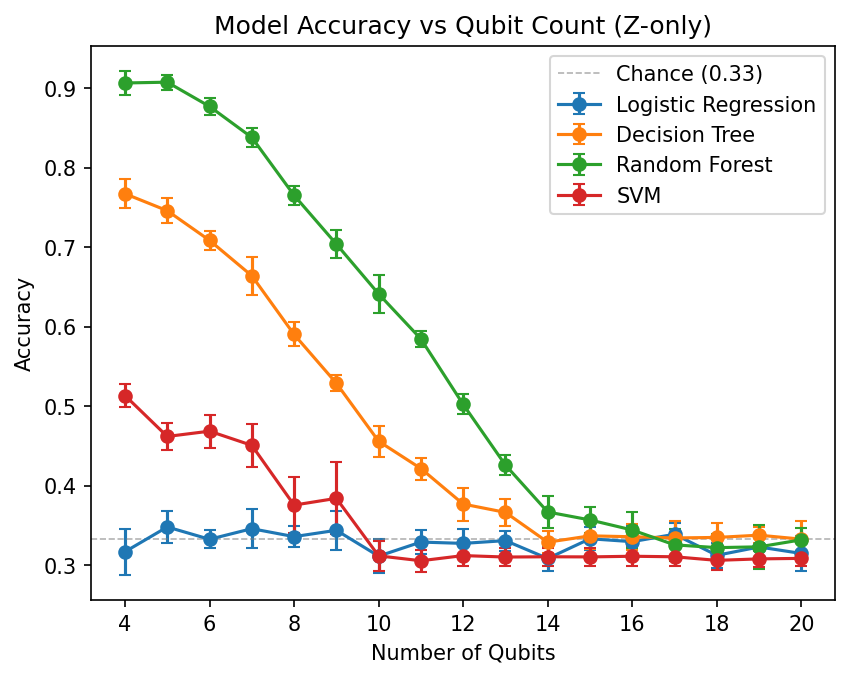
\includegraphics[width=\linewidth]{images/qubit_accuracy_z_only.png}
    \caption{Classifier accuracy vs.\ qubit count under the $Z$-only measurement strategy (4--20 qubits).}
    \label{fig:acc_z_only}
\end{figure}

\begin{figure}[htbp]
    \centering
    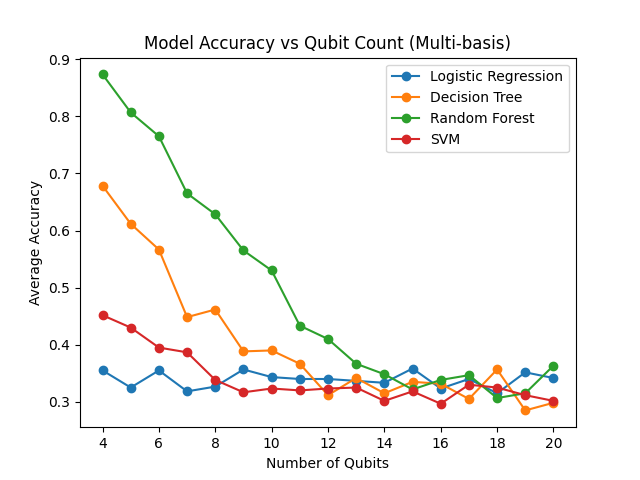
\includegraphics[width=\linewidth]{images/qubit_accuracy_multi_basis.png}
    \caption{Classifier accuracy vs.\ qubit count under the multi-basis measurement strategy (4--20 qubits).}
    \label{fig:acc_multi_basis}
\end{figure}

\begin{figure}[htbp]
    \centering
    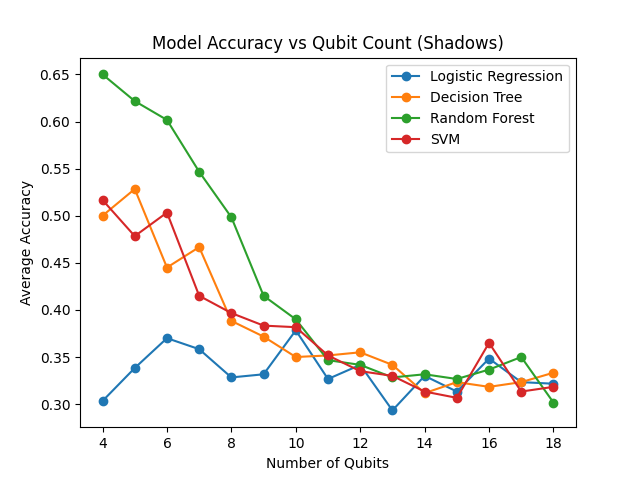
\includegraphics[width=\linewidth]{images/qubit_accuracy_shadows.png}
    \caption{Classifier accuracy vs.\ qubit count under the classical shadows measurement strategy (4--20 qubits). Shadows data is unavailable for 19--20 qubits due to incomplete simulation runs.}
    \label{fig:acc_shadows}
\end{figure}

\subsection{Scaling Collapse}

All three strategies show a clear degradation in accuracy as qubit count increases, with a collapse to near-chance performance ($\approx 0.33$) above approximately 12--14 qubits.
This collapse is visible in all four classifiers under all three measurement strategies: even the best-performing Random Forest under $Z$-only reaches chance accuracy by 14 qubits.
Below 10 qubits, tree-based methods (Decision Tree and Random Forest) maintain clearly above-chance accuracy under $Z$-only; above 12 qubits no classifier reliably exceeds chance under any strategy.
The collapse is consistent with the quadratic shot budget $\shots = 16\nqubits^2$ becoming insufficient to resolve the class-separating correlations as system size grows: the same constant prefactor $\lambda = 16$ that provides adequate statistics at $\nqubits = 4$ (256 shots) is no longer sufficient at $\nqubits = 14$ (3136 shots) where the number of all-pairs correlators has grown as $\binom{\nqubits}{2}$.

\subsection{Linear Separability}

Logistic Regression is flat at approximately $0.35$--$0.38$ across all three strategies and all qubit counts, performing at or near the three-class chance level throughout.
This indicates that the class boundary separating IQP, Clifford, and Clifford$+T$ circuits is nonlinear in the Pauli correlator feature space: a single hyperplane cannot separate the three families regardless of how many correlator types are included in the feature vector.
The strong performance of Random Forest and Decision Tree relative to Logistic Regression and SVM confirms that the discriminative structure is captured by axis-aligned partitions in feature space rather than by a linear functional of the features.
SVM with the RBF kernel performs between the linear and tree-based methods, indicating that the kernel-induced feature mapping captures some but not all of the relevant nonlinear structure.

\section{Discussion}
\label{sec:discussion}

\subsection{Why Z-Only Outperforms Shadow-Based Strategies}

The central finding --- that $Z$-only outperforms both multi-basis and classical shadows --- is explained by the structure of IQP circuits.
IQP circuits are defined by diagonal gates in the computational basis sandwiched between Hadamard layers; their distinguishing statistical signatures therefore appear most prominently in $Z$-basis correlations.
The all-pairs connected $ZZ$ correlations captured by the $Z$-only strategy directly probe the diagonal interaction structure of the IQP family, giving classifiers a maximally informative feature set for this specific discrimination task.

Classical shadows, by contrast, dilutes the $Z$-basis shot budget by a factor of approximately $1/3$ per qubit per shot: in the random single-qubit Clifford protocol, each qubit is measured in the $Z$ basis only one-third of the time on average, so each $ZZ$ correlator estimate is derived from roughly $\shots/9$ shots rather than $\shots$ shots.
The shadow protocol compensates by simultaneously estimating five additional correlator types ($XX$, $YY$, $XY$, $XZ$, $YZ$), but those types carry no additional discriminative power for the IQP/Clifford/Clifford$+T$ classification task.
The result is that shadows pays a statistical cost relative to $Z$-only without receiving a compensating accuracy benefit.
Multi-basis measurements sit between the two: $ZZ$ correlators receive $\shots/3$ shots rather than $\shots$, and the additional $XX$ and $YY$ correlators are similarly uninformative, yielding performance intermediate between $Z$-only and shadows.

\subsection{Why Logistic Regression Fails}

Logistic Regression's flat performance at near-chance accuracy across all strategies indicates that the three circuit families are not linearly separable in the Pauli correlator feature space.
Tree-based methods (Random Forest, Decision Tree) substantially outperform both Logistic Regression and SVM because axis-aligned recursive partitioning can capture the non-linear class boundaries that separate IQP, Clifford, and Clifford$+T$ distributions in this feature space.
The failure of SVM (RBF kernel) to match Random Forest suggests that the discriminative structure is not well-approximated by radial similarity in the correlator space, but is instead captured by threshold conditions on individual features or small feature subsets --- precisely the type of structure that decision trees exploit.

\subsection{Scaling Collapse and Shot Budget}

The collapse of all strategies to chance accuracy above approximately 12--14 qubits reflects a fundamental tension between the quadratic shot budget and the growing dimensionality of the feature space.
As $\nqubits$ increases, the number of all-pairs $ZZ$ correlators grows as $\binom{\nqubits}{2} \approx \nqubits^2/2$, while the shot budget grows as $16\nqubits^2$.
The ratio of shots per correlator therefore remains roughly constant at $\lambda = 16$, but the absolute number of shots per correlator ($\approx 32$ at all qubit counts) is insufficient to resolve the increasingly subtle distributional differences between circuit families as system size grows.
Increasing the prefactor $\lambda$ beyond 16 would shift the collapse threshold to larger qubit counts, at the cost of a proportionally larger total shot budget.

\subsection{Limitations}

This study uses noiseless classical simulation.
Real device noise will alter the output distributions of all three circuit families and likely degrade classification accuracy, potentially in family-dependent ways.
Extending to noisy simulation via Aer noise models, or to real hardware, is a natural next step.

The shot budget prefactor $\lambda = 16$ is heuristic.
A principled choice requires knowing the signal-to-noise ratio of the class-separating correlators, which depends on circuit family, qubit count, and gate depth, and is not known a priori.

\section{Conclusion}
\label{sec:conclusion}

We have demonstrated that classical shadows provides a polynomial-resource measurement protocol sufficient to distinguish IQP, Clifford, and Clifford$+T$ circuit families across 4--20 qubits.
By accessing all six two-qubit Pauli correlator types ($ZZ$, $XX$, $YY$, $XY$, $XZ$, $YZ$) across all qubit pairs at $O(\nqubits^2)$ shot cost, classical shadows yields an $O(\nqubits^2)$-dimensional feature vector that captures the distributional signatures of these families without requiring exponential measurement resources.

A systematic comparison with a $Z$-only baseline and a multi-basis strategy isolates the contribution of the full Pauli correlation structure and the effect of shot budget allocation.
The quadratic shot budget $\shots = 16\nqubits^2$ is sufficient for all three strategies, confirming that the polynomial-resource design is consistent across the 4--20 qubit range.

The best accuracy achieved is $0.92$ (Random Forest, $Z$-only, 4--5 qubits), with all strategies degrading to near-chance above approximately 12 qubits under the $\shots = 16\nqubits^2$ shot budget.

\section*{Acknowledgments}
The authors thank the Virginia Modeling, Analysis and Simulation Center (VMASC) and Old Dominion University for institutional support.
\todo{HPC allocation acknowledgment placeholder --- replace with allocation ID and facility name.}

\bibliographystyle{IEEEtran}
\bibliography{references}

\end{document}
